\chapter{Specyfikacja gramatyki}

% TODO 
% specyfikację gramatyki języka w notacji wybranego przez siebie narzędzia 
% wzorowane na Rozdziale 1 oraz Dodatku „Przewodnik języka C” (Sekcja „Gramatyka”) 
% książki „Język C”, B. Kernighan, D. Ritchie.

\section{Lexer}
Poniżej zostały przedstawione tokeny obsługiwane przez nasz translator.

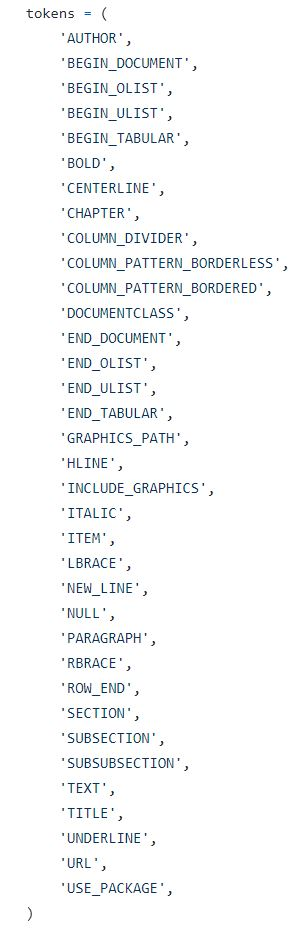
\includegraphics{tokens.JPG}


Tokeny odpowiadają następującym wyrażeniom regularnym:

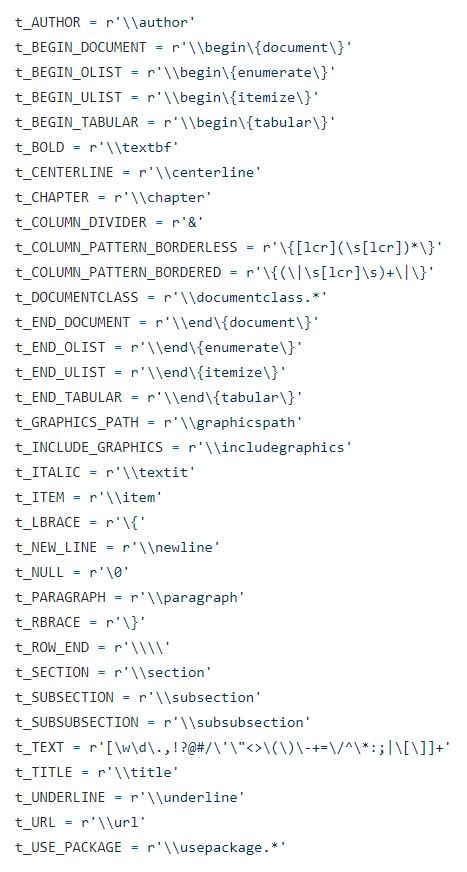
\includegraphics{tokens_regex.JPG}


Zdefininiowane zostały jak jest to pokazane poniżej.

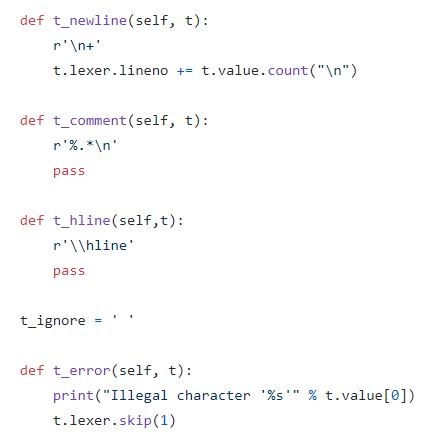
\includegraphics{tokens_def.JPG}

Należy zauważyć, że cała zawartość między znacznikiem \% w formacie LaTeX, odpowiadającemu początkowi komentarza, do nowej linii, 
zostaje pominięta.

\section{Parser}

Każdy z dokumentów HTMLa musi zawierać znaczniki typowe dla tego formatu, których nie znajdziemy w dokumentach LaTeX. Są to: html,
head, body. Jako odpowienik sekcji head przyjęliśmy usepackage, a body odpowiada begin i end document.

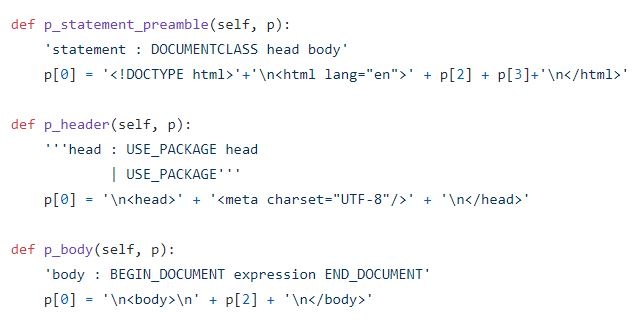
\includegraphics{preamble.JPG}

\subsection{Obsługa tekstu}

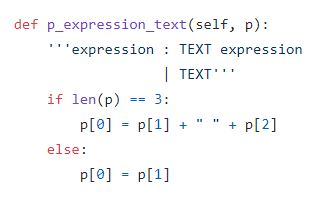
\includegraphics{expression_text.JPG}

\subsection{Formatowanie tekstu}

Nasz translator umożliwia pogrubienie, kursywa, podkreślenie, wyśrodkowanie tekstu oraz utworzenie paragrafu. Możliwe jest mieszanie
stylów formatowania, np. pogrubienie z podkreśleniem. Według nowych zaleceń, do pogrubienia tekstu w HTMLu powinno się stosować znacznik
"strong", a do kursywy "em".

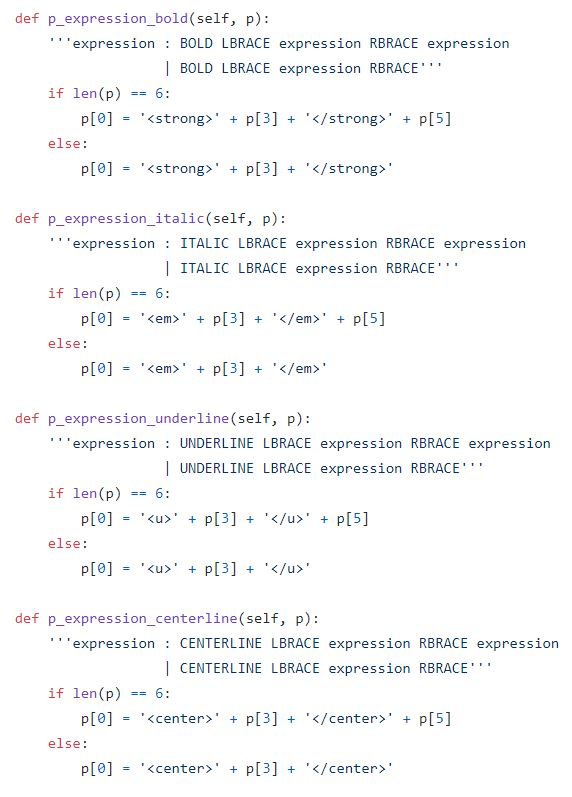
\includegraphics{bold_italic_underline_centerline.JPG}

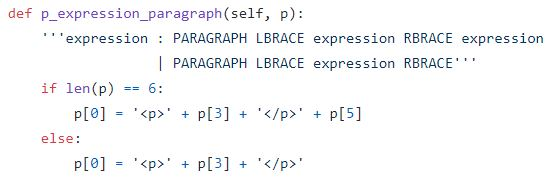
\includegraphics{paragraph.JPG}


Kolejną funkcjonalnością jest możliwość obsługi rozdziałów, sekcji i podsekcji parsując znaczniki chapter, section, subsection, 
subsubsection.


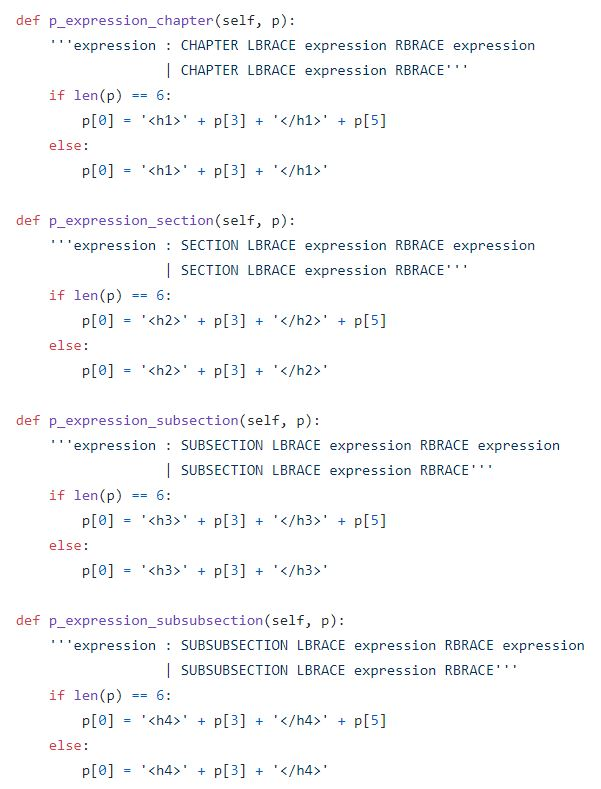
\includegraphics{chapter_section.JPG}


Przejście do nowej linii (hard break) jest obsłużony poleceniem newline.

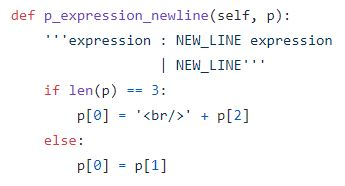
\includegraphics{newline.JPG}


Translator parsuje również znacznik title odpowiadjący z utworzenie tytułu.

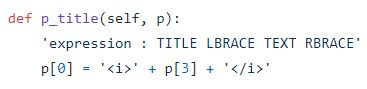
\includegraphics{title.JPG}

\subsection{Tabela}

\subsubsection{Z obramowaniem}

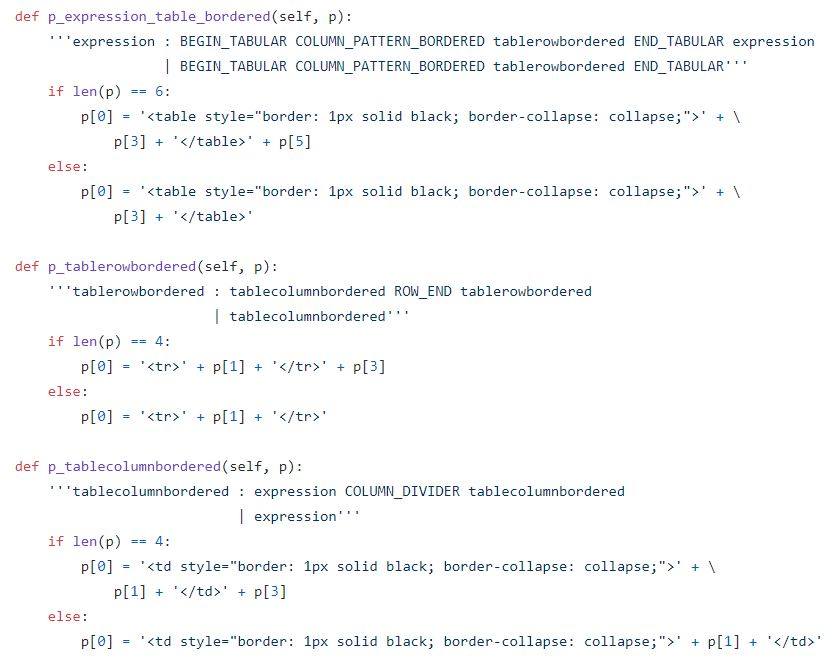
\includegraphics{table_bordered.JPG}

\subsubsection{Bez obramowania}

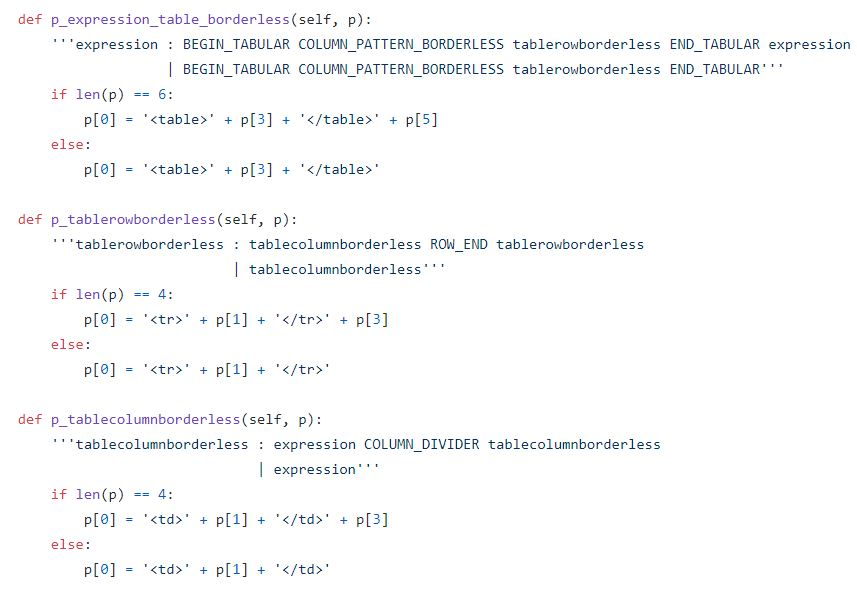
\includegraphics{table_borderless.JPG}


\subsection{Wyliczenie}

Konstrukcja parsera wyliczeń umożliwia wykonywanie zagnieżdżeń.

\subsubsection{Uporządkowane}

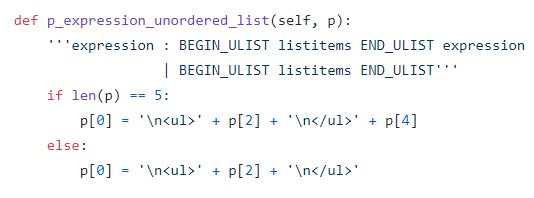
\includegraphics{unordered_list.JPG}

\subsubsection{Nieuporządkowane}

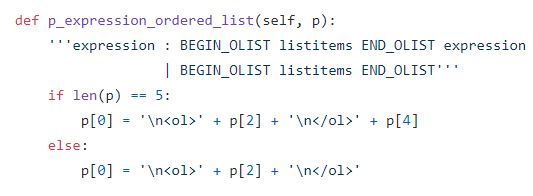
\includegraphics{ordered_list.JPG}

\subsection{Grafika}

Umieszcznie grafiki jest możliwe dzięki znacznikowi "includegraphics" w LaTeX, który jest parsowany na znacznik "img" w HTML, gdzie 
atrybut :src" stanowi ścieżka do pliku umieszczona w nawiasach wąsatych w dokumencie LaTeX.

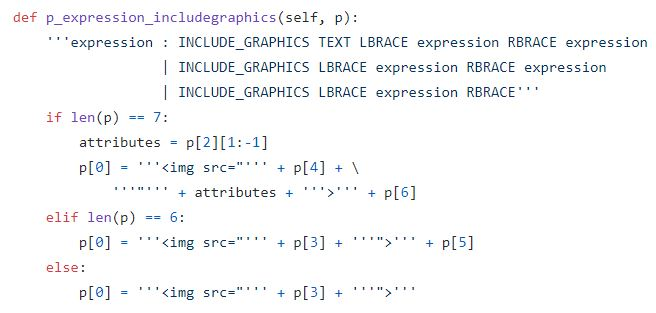
\includegraphics{includegraphics.JPG}

\subsection{Hiperłącze}

Zamieszczenie hiperłącza w formacie LaTeX jest możliwe dzięki znacznikowi "url", zawierającego w nawiasach wąsatych adres do strony.
Parsowanny jest on na HTMLowy znacznik "a" z atrybutem "href" zawierającego adres.

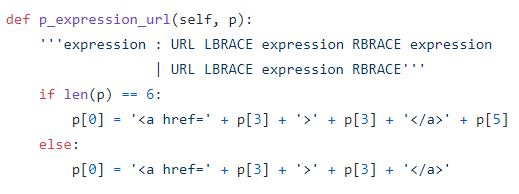
\includegraphics{url.JPG}